\documentclass[a4paper,12pt]{article}
\usepackage[top = 2.5cm, bottom = 2.5cm, left = 2.5cm, right = 2.5cm]{geometry}
\usepackage[T1]{fontenc}
\usepackage[utf8]{inputenc}
\usepackage{multirow} 
\usepackage{booktabs} 
\usepackage{graphicx}
\usepackage[spanish]{babel}
\usepackage{setspace}
\setlength{\parindent}{0in}
\usepackage{float}
\usepackage{fancyhdr}
\usepackage{amsmath}
\usepackage{amssymb}
\usepackage{amsthm}
\usepackage[numbers]{natbib}
\newcommand\Mycite[1]{%
	\citeauthor{#1}~[\citeyear{#1}]}
\usepackage{graphicx}
\usepackage{subcaption}
\usepackage{booktabs}
\usepackage{etoolbox}
\usepackage{minibox}
\usepackage{hyperref}
\usepackage{xcolor}
\usepackage[skins]{tcolorbox}
%---------------------------

\newtcolorbox{cajita}[1][]{
	 #1
}

\newenvironment{sol}
{\renewcommand\qedsymbol{$\square$}\begin{proof}[\textbf{Solución.}]}
	{\end{proof}}

\newenvironment{dem}
{\renewcommand\qedsymbol{$\blacksquare$}\begin{proof}[\textbf{Demostración.}]}
	{\end{proof}}

\newtheorem{problema}{Problema}
\newtheorem{definicion}{Definición}
\newtheorem{ejemplo}{Ejemplo}
\newtheorem{teorema}{Teorema}
\newtheorem{corolario}{Corolario}[teorema]
\newtheorem{lema}[teorema]{Lema}
\newtheorem{prop}{Proposición}
\newtheorem*{nota}{\textbf{NOTA}}
\renewcommand\qedsymbol{$\blacksquare$}
\usepackage{svg}
\usepackage{tikz}
\usepackage[framemethod=default]{mdframed}
\global\mdfdefinestyle{exampledefault}{%
linecolor=lightgray,linewidth=1pt,%
leftmargin=1cm,rightmargin=1cm,
}




\newenvironment{noter}[1]{%
\mdfsetup{%
frametitle={\tikz\node[fill=white,rectangle,inner sep=0pt,outer sep=0pt]{#1};},
frametitleaboveskip=-0.5\ht\strutbox,
frametitlealignment=\raggedright
}%
\begin{mdframed}[style=exampledefault]
}{\end{mdframed}}
\newcommand{\linea}{\noindent\rule{\textwidth}{3pt}}
\newcommand{\linita}{\noindent\rule{\textwidth}{1pt}}

\AtBeginEnvironment{align}{\setcounter{equation}{0}}
\pagestyle{fancy}

\fancyhf{}









%----------------------------------------------------------
\lhead{\footnotesize Álgebra Moderna}
\rhead{\footnotesize  Rudik Roberto Rompich}
\cfoot{\footnotesize \thepage}


%--------------------------

\begin{document}
 \thispagestyle{empty} 
    \begin{tabular}{p{15.5cm}}
    \begin{tabbing}
    \textbf{Universidad del Valle de Guatemala} \\
    Departamento de Matemática\\
    Licenciatura en Matemática Aplicada\\\\
   \textbf{Estudiante:} Rudik Roberto Rompich\\
   \textbf{Correo:}  \href{mailto:rom19857@uvg.edu.gt}{rom19857@uvg.edu.gt}\\
   \textbf{Carné:} 19857
    \end{tabbing}
    \begin{center}
        MM2035 - Álgebra Moderna - Catedrático: Ricardo Barrientos\\
        \today
    \end{center}\\
    \hline
    \\
    \end{tabular} 
    \vspace*{0.3cm} 
    \begin{center} 
    {\Large \bf  Tarea 13
} 
        \vspace{2mm}
    \end{center}
    \vspace{0.4cm}
%--------------------------

Problemas 1, 2, 3, 4, 5, 6 y 7, sección 5.8


\begin{problema}[Problema 1]
    In $S_5$ show that $(1 2)$ and $(1 2 3 4 5)$ generate $S_5$.
    \begin{dem}
       Por cálculo directo (de derecha a izquierda), usamos la expresión $(1 2 3 4 5)^{j}t(1 2 3 4 5)^{-j}$, donde $1\leq j\leq 5$, tal que:

       \begin{itemize}
        \item $(1 2 3 4 5)^{1}(1 2)(1 2 3 4 5)^{-1} = (1 2 3 4 5)(1 2)(54321)=(23) $
        \item $(1 2 3 4 5)^2(1 2)(54321)^2=(34) $
        \item $(1 2 3 4 5)^3(1 2)(54321)^3=(45) $
        \item $(23)(1 2)(23)=(13) $
        \item $(34)(13)(34)= (14)$
        \item $(45)(14)(45)= (15)$
        \item $(45)(34)(45)= (35)$
        \item $(35)(23)(35)= (25)$
        \item $(34)(23)(34)= (24)$
       \end{itemize}
       Como generamos todos los 2-ciclos en $S_5$, podemos generar $S_5$.
    \end{dem}

\end{problema}

\begin{problema}[Problema 2]
    In $S_5$ show that $(1 2)$ and $(13245)$ generate $S_5$.
    \begin{dem}
        Por cálculo directo (de derecha a izquierda), usamos la expresión $(13245)^{j}t(13245)^{-j}$, donde $1\leq j\leq 5$, tal que:
 
        \begin{itemize}
         \item $(13245)^{1}(1 2)(13245)^{-1} = (13245)(1 2)(54231)=(34)$
         \item $(13245)(34)(54231)=(25)$
         \item $(13245)(25)(54231)=(14)$
         \item $(13245)(14)(54231)=(35)$
         \item $(25)(12)(25)=(15)$
         \item $(35)(15)(35)=(13)$
         \item $(35)(13)(35)=(45)$
         \item $(35)(25)(35)=(23)$
         \item $(34)(23)(34)=(24)$
        \end{itemize}
        Como generamos todos los 2-ciclos en $S_5$, podemos generar $S_5$.
     \end{dem}
 
\end{problema}


\begin{problema}[Problema 3]
    If $p>2$ is a prime, show that (1 2) and $(2 \cdots p-1 p)$ generate $S_p$.
    \begin{dem}
        Directamente de un teorema ya demostrado, en donde $S_n$ es generado por $(1,2)$ y $(1,2,\cdots,n)$. Entonces este problema es un caso particular para números primos. 
    \end{dem}
\end{problema}




\begin{problema}[Problema 5]
    Show that the following polynomials over $\mathbb{Q}$ are irreducible and have exactly two nonreal roots.
    \begin{enumerate}
        \item $p(x)=x^3-3 x-3$
        \begin{sol}
            Por el criterio de Eisenstein con $p=3$, $p(x)$ es irreducible en $\mathbb{Q}$. La derivada de este polinomio: 
            $$p'(x)=3x^2-3$$
            Para encontrar los máximos y mínimos igualadas a cero, tal que:
            $$x^2=\frac{3}{3}\implies x=\pm 1$$
            Lo que nos permite concluir que tiene dos raíces imaginarias.
        \end{sol}
        \item $p(x)=x^5-6 x+3$
        \begin{sol}
            Por el criterio de Eisenstein con $p=3$, $p(x)$ es irreducible en $\mathbb{Q}$. La derivada de este polinomio: 
            $$p'(x)=5x^4-6$$
            Para encontrar los máximos y mínimos igualadas a cero, tal que:
            $$x^4=\frac{6}{5}\implies x=\pm \sqrt[4]{\frac{6}{5}}$$
            Lo que nos permite concluir que tiene dos raíces imaginarias.
        \end{sol}
        \item $p(x)=x^5+5 x^4+10 x^3+10 x^2-x-2$.
        \begin{sol}
            A primera vista no podemos usar Eisenstein, pero si usamos $p(x-1)$, tenemos: 
            \begin{align*}
                p(x-1) &= (x-1)^5+5(x-1)^4+10 (x-1)^3+10 (x-1)^2-(x-1)-2\\
                       &= (x-1)^2[(x-1)^3+5(x-1)^2+10(x-1)+10]-(x-1)-2\\
                       &= (x-1)^2[(x-1)[(x-1)^2+5(x-1)+10]+10]-(x-1)-2\\
                       &= (x-1)^2[(x-1)(x^2+3x+6)+10]-(x-1)-2\\
                       &= (x-1)^2[x^3+2x^2+3x+4]-(x-1)-2\\
                       &= x^5-5x+4-(x-1)-2\\
                       &= x^5-6x+3
            \end{align*}
            Este polinomio es irreducible por el inciso 2, entonces $p(x)$ también es irreducible. Además, también tiene 2 raíces imaginarias por el mismo argumento, ya que $(x-1)$ solo es un desplazamiento en el eje $x$ y la forma se preserva. 
        \end{sol}
    \end{enumerate}

\end{problema}


\begin{problema}[Problema 6]
    What are the Galois groups over $Q$ of the polynomials in Problem 5?
    \begin{dem}
        Por teorema 5U,
        \begin{enumerate}
            \item Grupo de Galois sobre $\mathbb{Q}$ es $S_3$ ya que $gr(p(x))=3$.
            \item Grupo de Galois sobre $\mathbb{Q}$ es $S_5$ ya que $gr(p(x))=5$.
            \item Grupo de Galois sobre $\mathbb{Q}$ es $S_5$ ya que $gr(p(x))=5$.
        \end{enumerate}
    \end{dem}
\end{problema}

\begin{problema}[Problema 7]
    Construct a polynomial of degreee 7 with rational coefficients whose Galois group over $\mathbb{Q}$ is $S_7$. 
    \begin{sol}
        Sea $p(x)=x^7-10x^5+25x$. Por el criterio de Eisenstein con $p=5$, $p(x)$ es irreducible en $\mathbb{Q}$. Para determinar las raíces de este polinomio, por su complejidad, se optó por usar el lenguaje de programación \textbf{Mathematica} en donde además se graficaron las raíces en el plano complejo por medio del siguiente código: 
        \begin{figure}[H]
            \centering
            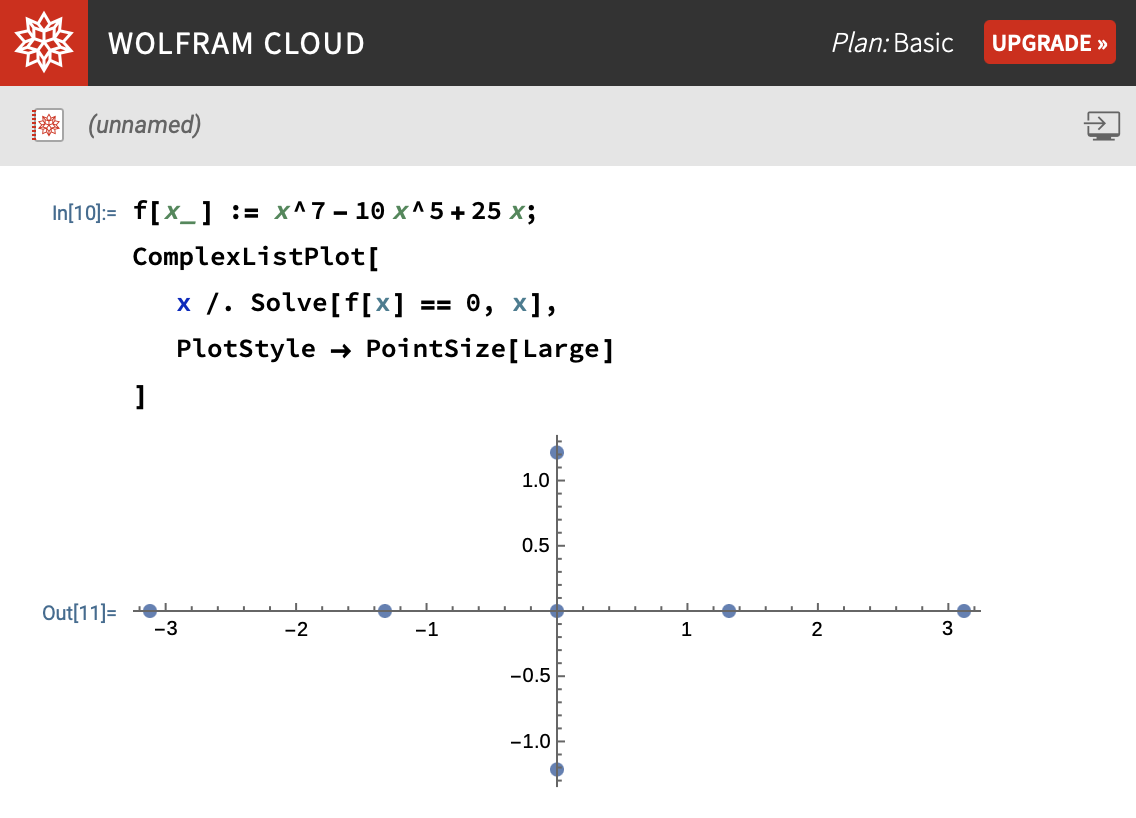
\includegraphics[scale=0.6]{Problemas/image1.png}
        \end{figure}
        Por lo que se comprueba que se tienen dos raíces imaginarias, además por el teorema 5U, $gr(p(x))=7$ entonces el grupo de Galois sobre $\mathbb{Q}$ es $S_7$.
    \end{sol}
\end{problema}



%---------------------------
%\bibliographystyle{apa}
%\bibliography{referencias.bib}

\end{document}